%%%%%%%%%%%%%%%%%%%%%%%%%%%%%%%%%%%%%%%%%%%%%%%%%%%%%%%%%%%%%%%%%%%%%%%%%%%%%%%%
%
% タイトル 安全な教育用マルチコプターの開発 
% バージョン 2016-12-22 (Thu) 初版
% 作成者 北山天斗,剱崎健太郎
% 作成場所 金沢工業高等専門学校
% 用途 卒論
%
%%%%%%%%%%%%%%%%%%%%%%%%%%%%%%%%%%%%%%%%%%%%%%%%%%%%%%%%%%%%%%%%%%%%%%%%%%%%%%%%

\documentclass[twocolumn,11pt]{sotsuken_abst}

% タイトル
\title{安全な教育用マルチコプターの開発}

\author{北山天斗$\cdot$剱崎健太郎(指導教員 伊藤恒平)}

%\urlstyle{rm}

\setcounter{page}{3}
\lhead{}
\chead{}
\rhead{{\sf 16・202}\\{\bf 機械工学科}}
\lfoot{}
\cfoot{{\sf-\ M-\thepage \ -}}
%\rfoot{}
\renewcommand{\headrulewidth}{3pt}
%\renewcommand{\footrulewidth}{1pt}

\begin{document}
%\layout
\maketitle
\thispagestyle{fancy}
\pagestyle{fancy}

\setlength{\baselineskip}{5.6truemm}
\kanjiskip=.07zw plus 3pt minus 3pt
\xkanjiskip=.07zw plus 3pt minus 3pt

%%%%%%%%%%%%%%%%%%%%%%%%%%%%%%%%%%%%%%%%%%%%%%%%%%%%%%%%%%%%%%%%%%%%%%%%%%%%%%%%

% 本文
\section{はじめに}

\subsection{研究背景}
当研究室では例年機械の制御について研究を行っており,今年度はマルチコプターを題材にする.
私達は学校という教育機関に所属する者として,機械制御を学ぶ上で役に立つものを作りたいと考えた.

\subsection{研究目的}
来年度以降の研究を円滑に進めること,プロペラによる負傷事故が多いため安全化を行うことを念頭に置き以下の目標を掲げた.

\begin{itemize}
	\item 機体の製作マニュアルを作成
	\item RaspberryPiでの制御実習環境の構築
	\item 機体を球形カバーで覆う
\end{itemize}


\section{ハードウェア開発の目標}
機体は強度や重量,製作費,メンテナンス性などを考慮し開発を行う.
また,機体の保護・安全化のため機体を覆う球体カバーの開発を行う.


\section{ハードウェアの仕様}
開発したマルチコプターの機体,球体についてそれぞれ仕様を以下に示す.
また,実際に製作したマルチコプターを図\ref{fig:multicopter}に示す.

\begin{figure}[htbp]
	\begin{center}
		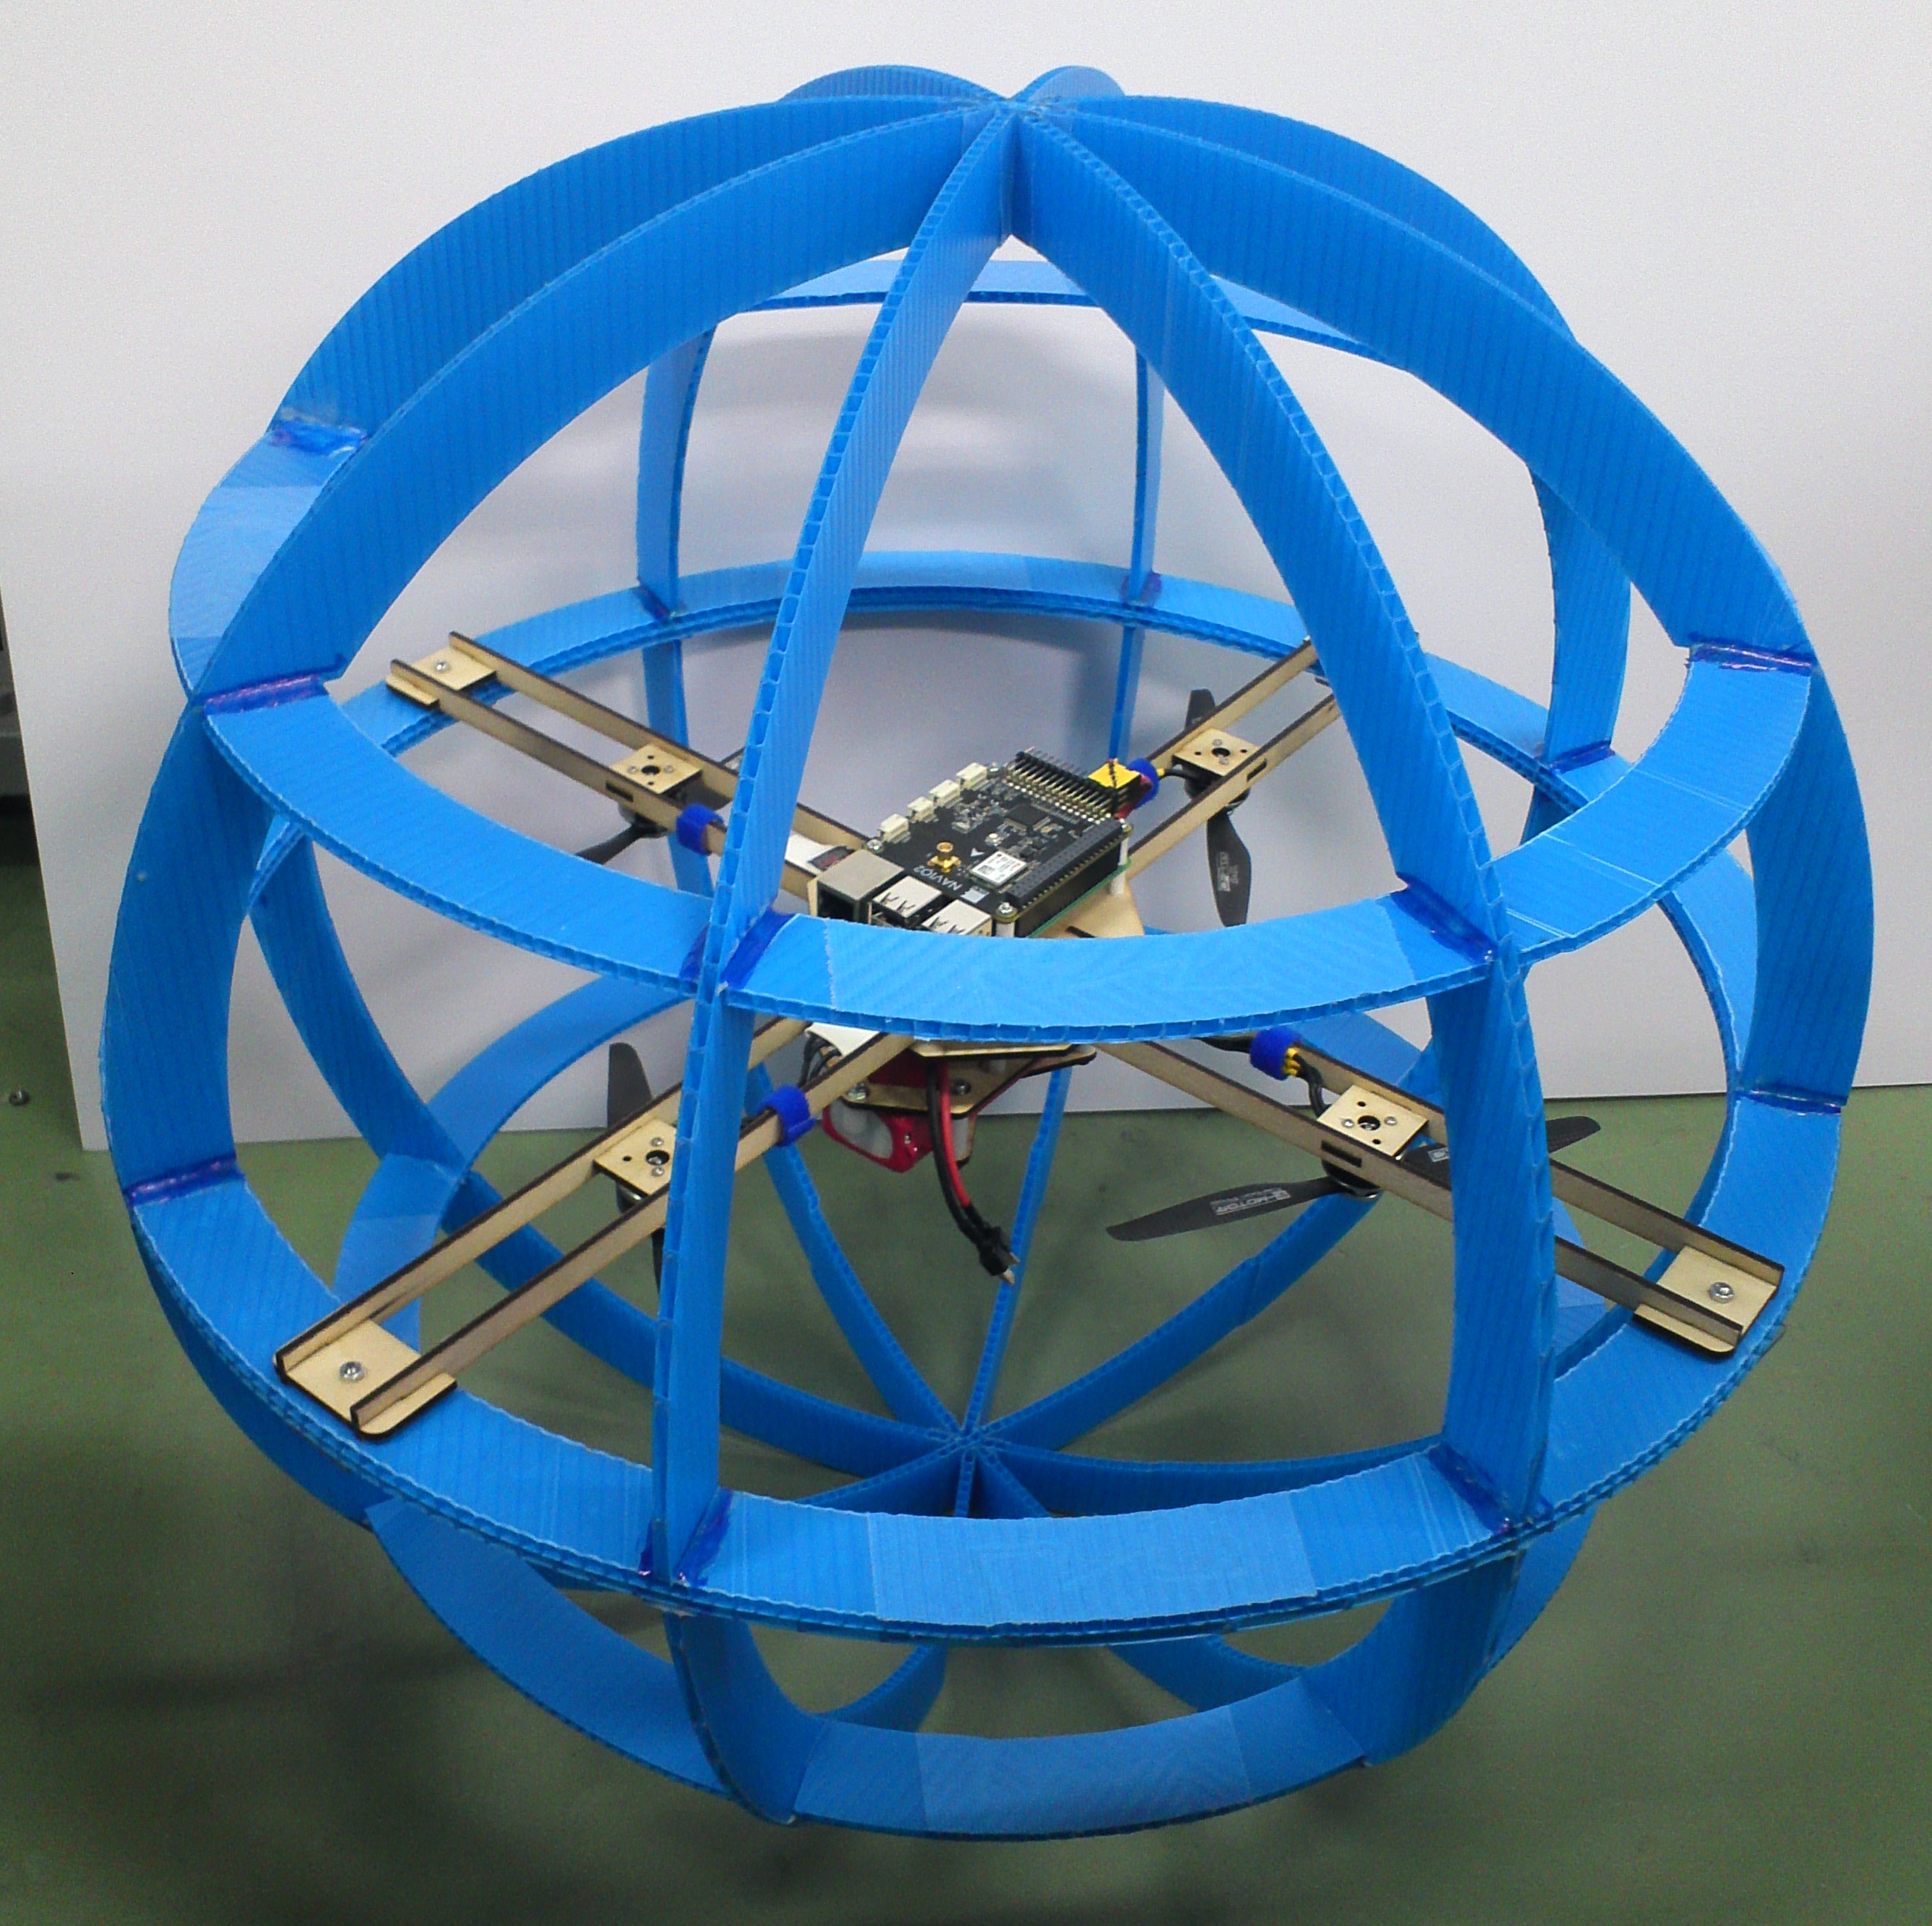
\includegraphics[width=50mm]{image/multicopter.jpg}
		\caption{マルチコプター}
		\label{fig:multicopter}
	\end{center}
\end{figure}

\subsection{機体}
厚さ3mmの木の板から切り出したパーツを主として使用している.
アームの長さが前後左右ともに500mm,高さが100mm,プロペラの中心間距離が275mm,重量は476gである.

モータはT-MOTOR製のMN1804,モータドライバ(ESC)はモータ付属のS12A,プロペラも同社製のP6x2prop-2PCS/PAIRを使用している.

\subsection{球体}
プラスチックダンボールから環を複数のパーツに分割したものを切り出し,これらを木組みの要領で組み立て直径510mmの骨組みの半球を形成する.
これを2つ組み合わせることで球体カバーとなる.
重量は223gである.


\section{ハードウェア開発の経緯}
ハードウェアが現在のものに至るまでの経緯について述べる.

\subsection{機体}
当初は機体全体をアルミを材料に製作していたが,塑性変形してしまうなどの問題があった.
そこで,アームをCFRPのパイプにしてみたが,CFRPは高価で加工難しいため現在のように木の板を材料とした機体に変更した.
また,木の板を材料にすることでレーザー加工機での機体製作が可能となった.

\subsection{球体}
当初は球体をスチレンボードで製作していた.
接合部を接着剤で固定していたところスチレンと紙が剥離し破壊してしまったため,接合部に木組み構造を取り入れた.
手作業による加工では時間がかかるため,パーツの切り出しをレーザー加工機で行うことにした.
これにより,製作時間が短縮でき加工精度も格段に増した.
しかし,幾度もの墜落により破損してしまったため,材料をプラスチックダンボールに変更した.

\subsection{結果}
レーザー加工機を使用することにより,機体・球体ともに簡単に製作が可能となった.
また,機体を球体カバーで覆ったことにより安全性の確保,機体の保護ができた.


\section{ソフトウェア開発の目標}
航空機力学の座標系\cite{config}に準じ,図\ref{fig:config}のように座標系を設定している.
角変位は右ねじの法則に従いx軸回りをロール,y軸回りをピッチ,z軸回りをヨーとする.
コンピュータにRaspberryPi3 ModelB,センサモジュールにNavio2,コントローラにDUALSHOCK3を使用する.
Navio2に搭載されている加速度センサ,ジャイロセンサ,地磁気センサにより,加速度・角度・角速度・方角などの情報を取得する.
DUALSHOCK3のスティック操作により操作を行う.

\begin{figure}[htbp]
	\begin{center}
		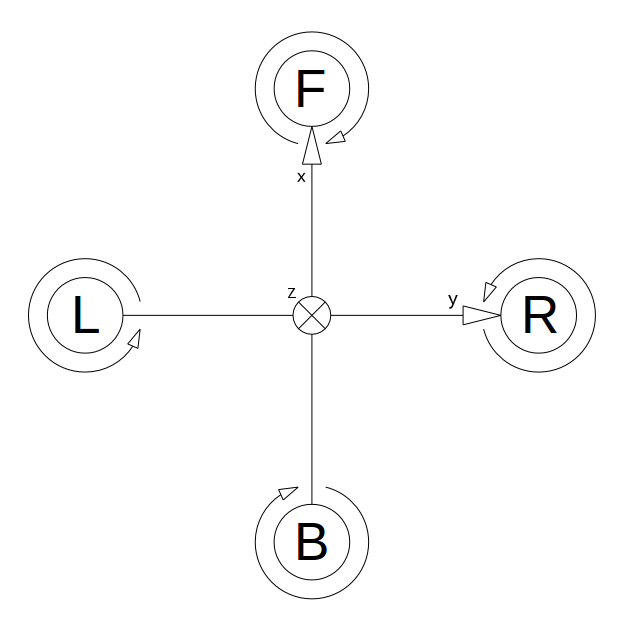
\includegraphics[width=50mm]{image/config.png}
		\caption{座標系の設定}
		\label{fig:config}
	\end{center}
\end{figure}


\section{ソフトウェア開発の経緯}
ソフトウェアが現在のものに至るまでの経緯について述べる.

\subsection{PID制御}
PID制御は目標値と現在の値の差に比例・積分・微分をそれぞれ行い,それらに補正値を掛けて足し合わせることで必要な制御量を求める制御方式である.\cite{pid}
当初はこのPID制御により機体の姿勢制御を行っていたが,球体に入れた際に姿勢が不安定になり離陸できないことが判明した.

\subsection{制御設計の見直し}
球体に入れた状態での離陸を可能とするため,最適レギュレータによる機体の姿勢安定化を考えた.
また,制御を確実なものにするため以下の作業を行った.

\begin{itemize}
	\item 加速度センサ・ジャイロセンサ・地磁気センサの校正
	\item 3次元CADデータを作成し,慣性モーメントなどの物理情報を取得
	\item 実験装置を製作し,各モータ・プロペラのPWM値と推力・モーメントの関係を調査
\end{itemize}

\subsection{最適レギュレータ}
飛行機の運動方程式に上記の実験から得られた値を用い,最適レギュレータの設計を行った.
最適レギュレータにより,各センサから得られた値をゼロに近づけることで機体の姿勢を水平に保つ.

\subsection{結果}
最適レギュレータにより,球体に入れた状態での離陸が可能となった.
最適レギュレータによる制御で飛行した際の角速度をグラフにしたものを図\ref{fig:gyro}に示す.

\begin{figure}[htbp]
	\begin{center}
		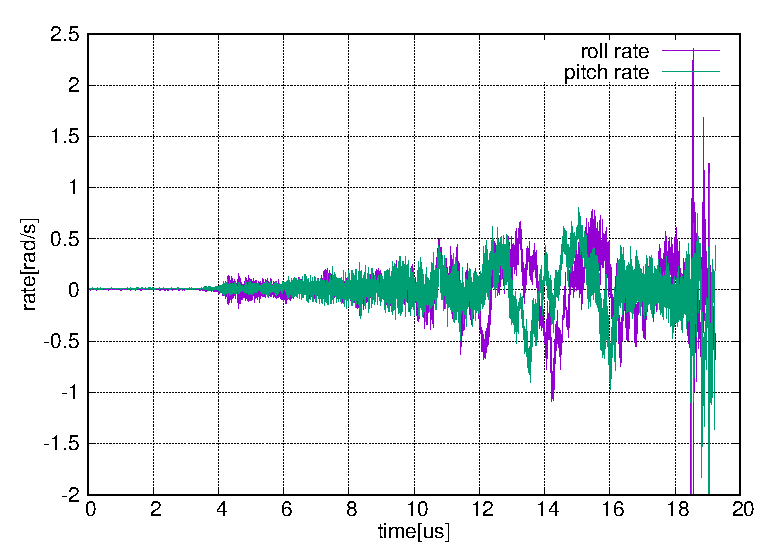
\includegraphics[width=60mm]{image/gyro.eps}
		\caption{飛行時の角速度}
		\label{fig:gyro}
	\end{center}
\end{figure}


\section{おわりに}

\subsection{今後の課題}
機体の上昇に必要な推力を減らすことで機体の姿勢制御に使用できる推力を増やすため,機体・球体の軽量化が必要である.

現在のプログラムにおいてセンサ情報の取得はサンプルプログラムを組み合わせて行っているため,プログラムの全容を把握しづらい.
そのため,センサ情報の取得を含めプログラム全体の制御式を見直す必要があると考える.

% 参考文献
\begin{thebibliography}{8}
\bibitem{config} 加藤寛一郎,大屋昭男,柄沢研治.(1982).航空機力学入門.14-14
\bibitem{pid} 森泰親.演習で学ぶPID制御.(2009).60
\end{thebibliography}

%%%%%%%%%%%%%%%%%%%%%%%%%%%%%%%%%%%%%%%%%%%%%%%%%%%%%%%%%%%%%%%%%%%%%%%%%%%%%%%%

\end{document}
